\documentclass[english]{article}
\usepackage{graphicx}


\makeatletter
\usepackage{url}

\makeatother

\usepackage{babel}
\begin{document}

\title{Netflix Challenge report}

\author{Yanqing Wu}

\maketitle

\section{Introduction}
\label{sec:intro}
\begin{itemize}
\item Introduce the topic and data
\item Explain the problem that you are solving 
\item Summarize your main contributions to solving the problem.
\end{itemize}


\section{Methodology}
\label{sec:method}
Describe the algorithms you used to solve the problem.
\subsection{Algorithm 1}
You could use subsections to describe different algorithms and/or improvements to them.


\section{Results}
\label{sec:result}
Describe your results. 
Include figures and quantitative facts proving that you method works (or not).
If you include figures or/and tables, always refer to them in the text, see table ~\ref{tab:table_example} and figure \ref{fig:figure_example}.
Make sure your figures are of good quality, have axis, ticks, labels, axis names and title. Also, the caption of the figure/table should contain sufficient information about the figure/table.
\begin{table}
\centering
\begin{tabular}{cc} 
\hline
heading1 &  heading 2  \\
\hline
value1,1 & value 2,1\\
value1,2 & value 2,2\\
\hline
\end{tabular}
\caption{This is an example of a table.} 
\label{tab:table_example}
\end{table}



\begin{figure*}
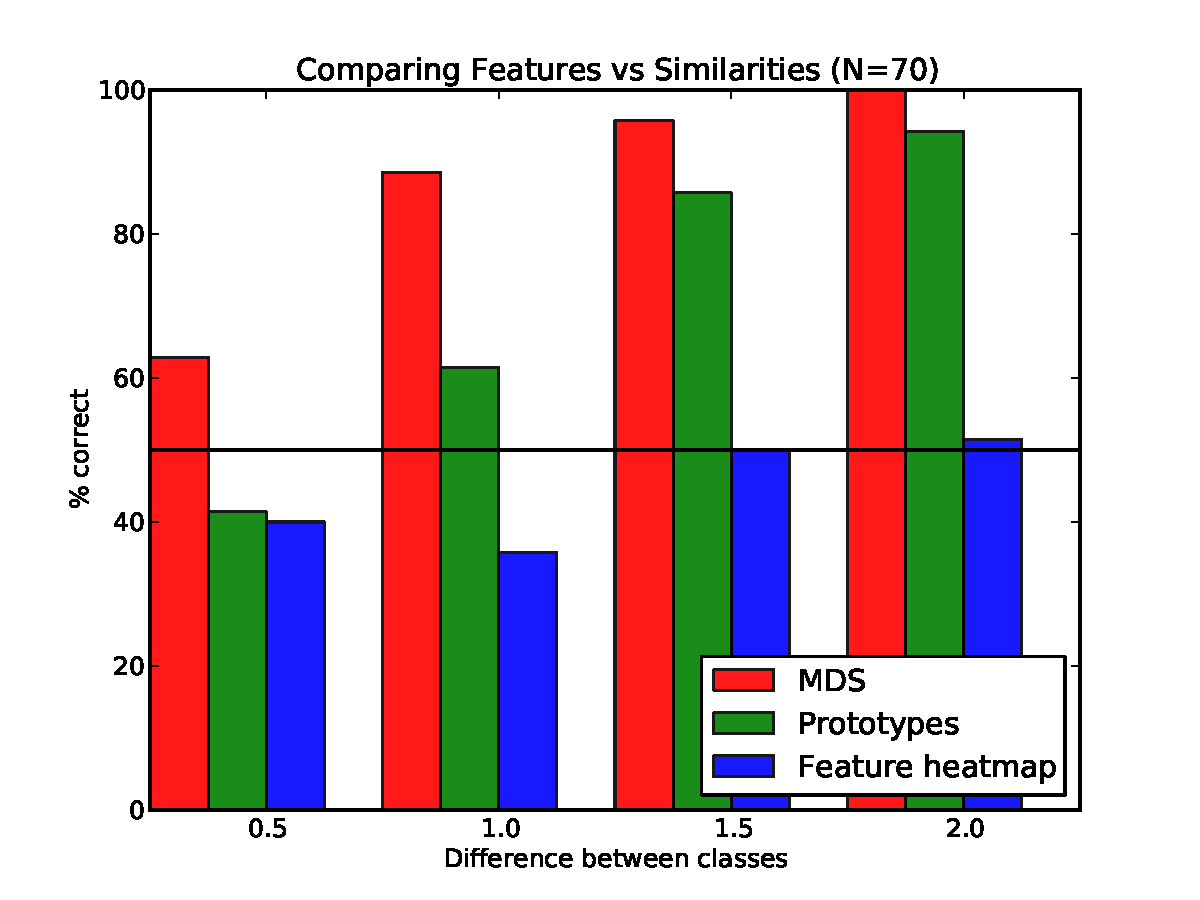
\includegraphics[width=0.9\linewidth]{exampleFig}
\caption{This is an exmaple of a figure.}
\label{fig:figure_example}
\end{figure*}

\section{Discussion}
\label{sec:disc}
Results can be compared to known results and placed in a broader context.
Provide a reflection on what has been concluded and how this was done.
Then give a further possible explanation of results.
This section can be joined with Conclusions.

\section{Conclusions and Future Work}
\label{sec:concl}
Summarize the problem you have been solving and the results.
Make statements.
Highlight interesting elements.
Discuss open issues, possible improvements, and new questions that arise from this work; formulate recommendations for further work.
This section can be joined with Discussion.






\bibliographystyle{plain}
\bibliography{template}

\end{document}
